Modern consumer software is increasingly relying on the ``cloud application'' model, where a browser- or mobile device-based client interacts with a functionally rich cloud service.
%
This model is prevalent in major systems like Facebook and GMail, as well as in smartphone and tablet ``apps'' like Instagram, Siri, or Dropbox.
%
For both developers and users, the economics are highly \mbox{attractive:} cloud-based applications offer ubiquitous access, transparent scaling, and easy deployment at low cost.

The hidden cost is that cloud apps introduce security, privacy, and availability risks. They store and process critical information remotely, so the impact of failures is higher in this model than for single-user desktop apps~\cite{web-failures-tr}.  This increases the importance of testing for cloud applications.

Rapid advances in development and deployment tools have significantly lowered the barrier to entry for developers, but these tools lack similarly advanced support for testing. Platform-as-a-service (PaaS) offerings, such as Google App Engine or Microsoft Azure, provide easy-to-use interfaces with automated deployment fully integrated into development environments.
%
However, testing tools for apps running on PaaS are still immature, test automation is limited, and developers are left with the laborious and error-prone task of manually writing large numbers of individual test cases.

Integration tests, which complement unit tests by checking that all the components of a fully deployed cloud application work together correctly, are especially tedious to write and set up in such an environment.
%
PaaS-based cloud applications typically use frameworks with a layered communication architecture and perform some processing at each of the layers. Writing a full integration test then requires to carefully craft an HTTP request that successfully passes through all application and framework layers and triggers the desired behavior, while being transformed from one representation to another at each step (e.g., from an HTTP request to JSON to language objects).

Spending precious developer time on testing for improving security and reliability is particularly unattractive in a viciously competitive environment.  Promoted by the ability to deploy virtually instantly and at low cost, the pressure is to use features to quickly acquire a large user base. Security and reliability testing is a long-term investment and does not pay off immediately, thus it is often deferred for later.
%
High-profile failures of cloud applications~\cite{bugs-linkedin,bugs-gmail} are thus likely to become a common occurrence, unless we can make testing easy and cheap.

We argue that {\em testing} must become at least as easy as {\em deploying} a new app. PaaS has made the latter easy, leaving the former just as hard to do as before.  A dedicated testing service must therefore become an integral component of PaaS.
%
Recent commercial test automation systems (CloudBees, Skytap, SOASTA, etc.) relieve developers of managing their own test infrastructure, but still require them to write test suites; we aim to further relieve developers of having to write individual tests.
%
Just as modern PaaS APIs spare developers from having to manage the building blocks of their applications, so should they spare developers from manually writing test cases, and instead offer means to automatically test apps based on only minimal input from developers.

The recent progress in automated test case generation and, in particular, symbolic execution takes an important step in this direction.  For a typical PaaS application like the example in Figure~\ref{fig:running-example}, a test case generator could use symbolic execution to automatically find HTTP packets that drive the execution to different parts of the code.
%
\begin{figure}
  \centering
  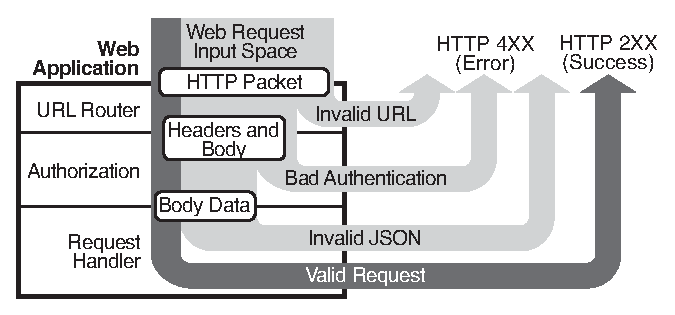
\includegraphics[width=0.7\textwidth]{paas/figures/web-flow}
  \caption{A sample cloud application.  Clients communicate with the server through web requests that traverse several layers inside the server before reaching the request handler logic.  From the total input space, most possible requests trigger errors in one of the processing layers (light arrows).  Only a small fraction of requests successfully traverses all layers and is handled inside the app (dark arrow).}
  \label{fig:running-example}
  \vspace{5pt}
\end{figure}
%
Unfortunately, these tools are challenging to apply to cloud apps: the number of execution paths successfully crossing all application layers is dwarfed by the vast number of possible error paths (dark vs.~light arrows in Figure~\ref{fig:running-example}).  Yet, most error paths are irrelevant to testing the high-level logic of the app itself (i.e., the innermost layer), because they test code that is part of the PaaS.

We leverage the modularity of each layer in modern web application stacks and introduce \textit{layered parameterized tests} (LPTs) for integration testing of PaaS-based cloud applications (Section~\ref{sec:paas:abstractions}).
%
LPTs describe families of integration tests (in the spirit of parameterized unit tests~\cite{tillmann-puts}) across several application layers. We rely on developer-provided \textit{onion objects} to describe the layering of the data abstractions in the application; onion objects encode the multiple interpretations of input data as, e.g., an HTTP request, a JSON object, etc.

For the automatic generation of thorough test cases from LPTs, we introduce \emph{layered symbolic execution} (LSE), an automated program analysis that is tailored for the layered structure of cloud applications (Section~\ref{sec:paas:layeredsymbex}).

Symbolic execution is a resource-intensive task, so we horizontally scale it in the cloud by introducing the first symbolic execution parallelization algorithm to demonstrate linear scalability in the number of nodes (Section~\ref{sec:paas:parsymbex}).

Finally, we present a design and early prototype for a PaaS-integrated parallel testing service based on LSE~(Section~\ref{sec:paas:fedsymbex}).

%%% Local Variables: 
%%% mode: latex
%%% eval: (visual-line-mode)
%%% fill-column: 1000000
%%% TeX-master: "main"
%%% End:
